%=====================================================================
\section{Centred and Uncentred Edits}
\label{app:edit}
%=====================================================================

\paragraph{Read strength}
The first thing the model does with an embedding is normalize it and project it into queries, keys and values.
For a unit direction $\mathbf u$ we define its read strength as $\big\|[W_Q; W_K; W_V]\,(\mathbf g \odot \mathbf u)\big\|$, with the layer-0 attention projections stacked and $\mathbf g$ the layer-0 RMSNorm scale, relative to the mean over 500 random unit directions; for Llama we also stack the MLP's gate and up projections, as the multilingual study did.
For a method we take the median over its edited tokens' directions $\cvec_t / \|\cvec_t\|$.

\begin{figure*}[t]
  \centering
  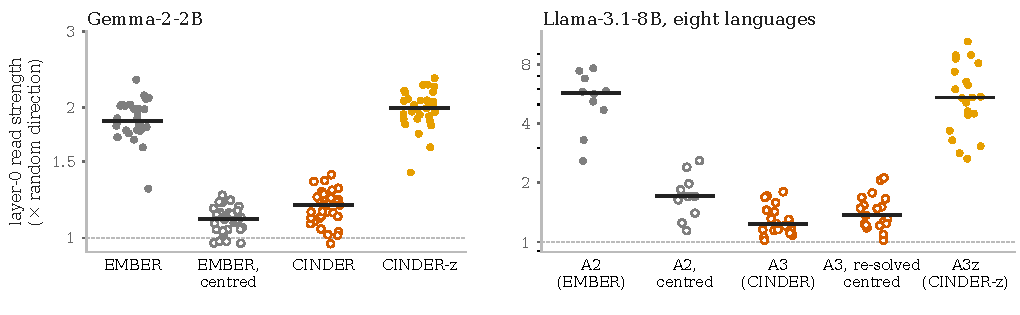
\includegraphics[width=\textwidth]{figures/read_decomposition.pdf}
  \caption{First-layer read strength of each edit relative to a random direction, per concept (dots) with medians (bars), on Gemma-2-2B (left) and the multilingual Llama-3.1-8B fits (right). Centring \ember{}'s dictionary brings its read strength down to \cinder{}'s on Gemma and most of the way on Llama; adding the mean term back (\cinderz{}, A3z) raises it again. Filled: uncentred edits; open: centred.}
  \label{fig:read}
\end{figure*}

\paragraph{The dictionary step does not depend on the metric}
Write $A_c = A - \mu_B\mathbf 1^{\top}$ for the centred embeddings.
The sharpened fit alternates $\tilde Z \leftarrow \tilde X Y^{\top}(YY^{\top}+\lambda I)^{-1}$ on $\tilde X = TA_c$ with a masked coefficient update, and \cinder{} maps the dictionary back as $T^{-1}\tilde Z$.

\begin{proposition}
\label{prop:metric}
For invertible $T$, $B \in \R^{d\times n}$, $Y \in \R^{k\times n}$ and $\lambda \ge 0$ with $YY^{\top} + \lambda I \succ 0$,
\begin{align*}
  &\arg\min_Z \|T(B - ZY)\|_F^2 + \lambda\|TZ\|_F^2 \\
  &\qquad = BY^{\top}(YY^{\top}+\lambda I)^{-1},
\end{align*}
independently of $T$.
\end{proposition}

\begin{proof}
$Z \mapsto \tilde Z = TZ$ is a bijection, and in $\tilde Z$ the objective $\|TB - \tilde ZY\|_F^2 + \lambda\|\tilde Z\|_F^2$ is strictly convex with minimizer $\tilde Z^* = TBY^{\top}(YY^{\top}+\lambda I)^{-1}$; hence $Z^* = T^{-1}\tilde Z^* = BY^{\top}(YY^{\top}+\lambda I)^{-1}$.
\end{proof}

\noindent At convergence of the fit, the mapped-back dictionary is therefore the Euclidean least-squares dictionary of the \emph{centred} embeddings, $Z_c = A_cY^{\top}(YY^{\top}+\lambda I)^{-1}$, for the affine model $\e_t \approx \mu_B + Z\mathbf y_t$ (on Gemma, $\|T^{-1}\tilde Z - Z_c\|/\|Z_c\| \le \expnum{0.008}$ in all \expnum{137} runs).
The coefficient step is where the metric matters: $Y$ is an $M$-orthogonal projection with $M = T^{\top}T$, so whitening chooses which tokens are grouped and how they are weighted.

\begin{proposition}
\label{cor:mean}
\cinderz{}'s dictionary (Eq.~\ref{eq:cinderz}) is $Z_z = Z_c + \mu_B\mathbf b^{\top}$ with $\mathbf b = (YY^{\top}+\lambda I)^{-1}Y\mathbf 1$, so its edit is $\cvec^{z}_t = \cvec_t + \beta_t\mu_B$ with $\beta_t = \sum_{i\in\Fc} b_i Y_{i,t}$.
\end{proposition}

\begin{proof}
Substitute $A = A_c + \mu_B\mathbf 1^{\top}$ in Eq.~\ref{eq:cinderz}.
\end{proof}

\noindent In the data, $\cvec^z_t - \cvec_t$ has at least \expnum{0.9995} of its energy along $\mu_B$ in every run (Gemma \expnum{137}, Llama \expnum{21}).
For a feature of width $w$ with same-sign coefficients of size about $1/\sqrt w$, $\beta_t \approx 1$ whatever $w$, so at $\delta = 1$ an uncentred edit subtracts roughly one full $\mu_B$ (observed median $\beta$: \ember{} \expnum{0.66}, \cinderz{} \expnum{0.56}, \cinder{} \expnum{0.05}; the edited tokens' own coordinate along $\mu_B$ is \expnum{1.06}).
The affine model also reconstructs raw embeddings better than the uncentred one (relative error \expnum{0.917} vs.\ \expnum{0.932}, 137 of 137 runs).

\paragraph{Where the read-strength gap comes from}
Concept means on Gemma-2-2B; $\perp\mu$: with $\hat\mu_B$ projected out of the edit.

\begin{center}
\footnotesize
\setlength{\tabcolsep}{2.5pt}
\begin{tabular}{@{}lcccc@{}}
\toprule
Edit & Read & $\hat\mu_B$ share & Read $\perp\mu$ & $\cos(\cvec_t,\e_t)$ \\
\midrule
\ember{} & \expnum{1.86} & \expnum{0.44} & \expnum{1.31} & \expnum{0.50} \\
\ember{}, centred $Z$ & \expnum{1.09} & \expnum{0.07} & \expnum{1.31} & \expnum{0.35} \\
\cinder{} & \expnum{1.18} & \expnum{0.05} & \expnum{1.32} & \expnum{0.30} \\
\cinderz{} & \expnum{1.99} & \expnum{0.48} & \expnum{1.32} & \expnum{0.50} \\
\bottomrule
\end{tabular}
\end{center}

\noindent \ember{} vs.\ \cinder{}: $+0.68$ read (27 of 27 concepts), but $-0.01$ once $\hat\mu_B$ is removed ($p = 0.44$), with the same Rayleigh ratio of the background covariance along the edit (\expnum{4.3} vs.\ \expnum{4.4}).
Across all edits, read strength follows the share along $\hat\mu_B$ (Spearman \expnum{0.75}) more closely than the background variance along the edit (\expnum{0.63}).
The mean term is also most of what aligns an uncentred edit with its token: with $\hat\mu_B$ removed from both, $\cos(\cvec_t, \e_t)$ is \expnum{0.31} for \ember{} and \expnum{0.29} for \cinder{} ($p = \expnum{0.15}$).
The read strength of the eigendirections of $\Sigma_B$ is U-shaped in their variance (top decile \expnum{1.08}, middle deciles \expnum{0.81--0.88}, bottom decile \expnum{1.59}, lowest 1\% \expnum{3.4}); strongly read directions concentrate on a few coordinates with a large first-layer normalization weight.
On Llama, A3z exceeds A3 by \expnum{$+4.48$} in read strength, of which \expnum{$+4.34$} is the mean term; $\hat\mu_B$ is read at \expnum{20.4$\times$}, so a \expnum{7\%} share suffices.
\paragraph{What the first layer does with the mean}
Setting the layer-0 normalization weight to one lowers $\hat\mu_B$'s read gain from \expnum{2.93$\times$} to \expnum{2.10$\times$} and the \ember{}--\cinder{} gap by \expnum{53\%}; zeroing its eight largest entries (\expnum{3.98--5.97}, against a median of \expnum{1.17}) lowers them to \expnum{1.74$\times$} and \expnum{75\%}; with $\hat\mu_B$ projected out, every edit is read at \expnum{1.28--1.35$\times$} under all three settings.
In the forward pass (50 tokens from 5 runs, each direction relative to random ones), the linear proxy predicts the measured layer-0 write well (Spearman \expnum{0.76--0.81}), and the mean and uncentred directions push far more change into the \emph{later} positions of the prompt (\expnum{2.1--4.3$\times$}, against \expnum{0.8--1.2$\times$} for the centred ones).
Yet at small perturbations the centred directions change the token's own next-token distribution more (KL \expnum{5.4$\times$} for \cinder{}, \expnum{3.9$\times$} for centred \ember{}, \expnum{1.6$\times$} for the mean direction); at $s = 1$ the directions are close.
The mean direction is thus ``read strongly'' in that it spreads into the context, not in that it changes what the model predicts at the token.

\subsection{The Mean Term on Its Own}
\label{app:mean}

\begin{figure*}[t]
  \centering
  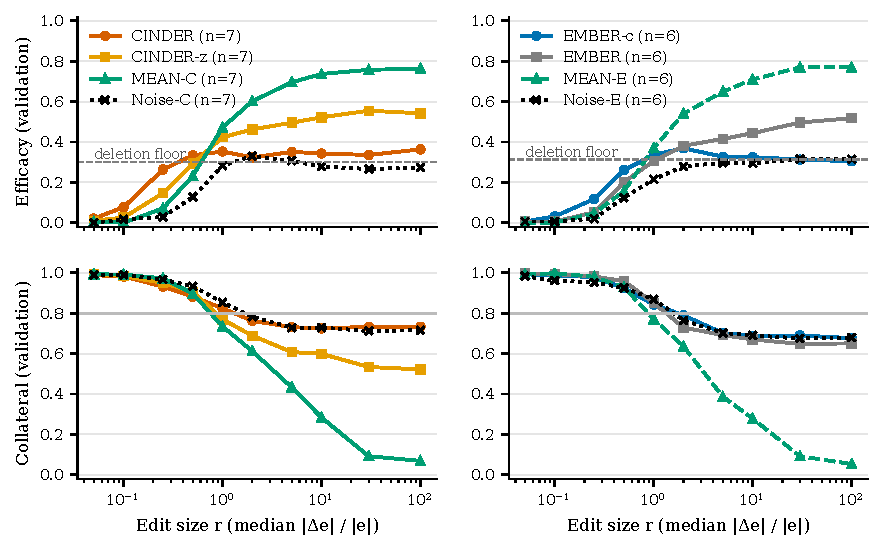
\includegraphics[width=0.85\textwidth]{figures/mean_curves.pdf}
  \caption{The mean term on its own (development runs, validation). Efficacy (top) and collateral (bottom) against edit size, mean over runs. Left: \cinder{}, \cinderz{}, the mean-only edit MEAN-C $= \beta^z_t\mu_B$ on \cinder{}'s tokens, and a random direction (7 runs). Right: \ember{}, \ember{} re-solved on centred embeddings (\ember{}-c), the mean-only edit MEAN-E on \ember{}'s tokens, and a random direction (6 runs). Dashed: deletion floor of the token set; grey: the collateral gate.}
  \label{fig:mean}
\end{figure*}

\paragraph{Design}
By Proposition~\ref{cor:mean}, \cinderz{}'s edit is \cinder{}'s plus $\beta_t\mu_B$, a term that carries no information about the concept.
We therefore evaluated that term alone (MEAN-C: $\e_t' = \e_t - \delta\beta^z_t\mu_B$ on \cinder{}'s tokens, with \cinderz{}'s own $\beta^z$), and the same split for \ember{} (\ember{}-c: \ember{}'s $Y$ and $\Fc$ with the dictionary re-solved on centred embeddings; MEAN-E: $\beta_t\mu_B$ with \ember{}'s coefficients), on the 8 development runs (Harry Potter, Ancient Rome and Valentine's Day; 7 with a \cinder{} edit, 6 with an \ember{} edit), over the same grid of $r$ and with the evaluation of App.~\ref{app:eval}.
The decompositions hold to a relative error of $10^{-4}$ in every run.
The test was pre-registered before any result (\path{results/paper_analysis/mean_edit/PREREG.md}); with three concepts, its statistics are descriptive.

\paragraph{The mean term erases by breaking the prompt}
Over $r \geq 1$, \cinderz{} removes \expnum{$+0.155$} more than \cinder{} (\expnum{7 of 7} runs), and the mean term alone removes more than \cinderz{} at every $r \geq 2$ (validation efficacy \expnum{0.60--0.76} vs.\ \expnum{0.46--0.55}) and more than a random direction of the same size (\expnum{$+0.48$} at $r \geq 10$, \expnum{7 of 7}; Figure~\ref{fig:mean}).
It does so by damaging the context: an unrelated multiple-choice question placed after a sentence with the edited word drops from \expnum{0.54} to \expnum{0.15--0.18} accuracy at $r \geq 10$, below chance, and collateral falls to \expnum{0.07}.
Across variants and sizes, efficacy above the deletion floor tracks this context damage (Spearman \expnum{0.54}, 63 points).
The centred edits destroy the words as completely at large $r$ (copy 0), yet stay near the floor with the context intact.
\ember{} shows the same pattern: centring its dictionary removes its large-$r$ gain (\expnum{$+0.097$} over $r \geq 1$, \expnum{6 of 6}) and its context damage, and raises efficacy at small edits (\expnum{$+0.07$} and \expnum{$+0.06$} at $r = 0.25$ and $0.5$).

\paragraph{Per unit of word damage, the centred edit erases most}
At the size where \expnum{90\%} of the edited words remain copyable, \cinder{} reaches efficacy \expnum{0.30}, \cinderz{} \expnum{0.20} and the mean term \expnum{0.13} (\ember{}-c \expnum{0.22}, \ember{} \expnum{0.15}, MEAN-E \expnum{0.11}); at \expnum{50\%} the three \cinder{} variants are equal.
Under the copy-gated rule, the mean term erases almost nothing (test efficacy \expnum{0.01}, against \expnum{0.12} for \cinder{} and \expnum{0.10} for \cinderz{}).
Under the collateral rule, however, it ties both (test $\Hthree$ \expnum{0.43} vs.\ \expnum{0.42} and \expnum{0.41}): collateral questions do not register damage to the rest of the prompt at $r \approx 0.5$.

\paragraph{Why the direction effect vanishes at $r = 1$}
The centred edits (\cinder{}, \ember{}-c, and \cinder{}'s direction on \ember{}'s tokens) reach a plateau near the deletion floor by $r \approx 0.5$--$1$, while \ember{} is still climbing, and keeps climbing past the plateau through generic damage.
On the 5 runs with all cells, centring \ember{}'s dictionary closes about a quarter of the gap to \cinder{}'s direction at $r = 0.5$ and nearly all of it at $r = 1$; the mean term becomes a net gain for \ember{} only at $r \geq 2$--$5$.
